\section{Graphics}
Det er mulgit at lave billeder på flere forskellige måder. Neden for er ses 3 billeder: figur \ref{fig::galaxy:top} på side \pageref{fig::galaxy:top} som er centreret, figur \ref{fig::galaxy:left} og figur \ref{fig::galaxy:right} på side \pageref{fig::galaxy:right} som er opstilt ved siden af hinanden.

\begin{figure}[ht]
    \centering
    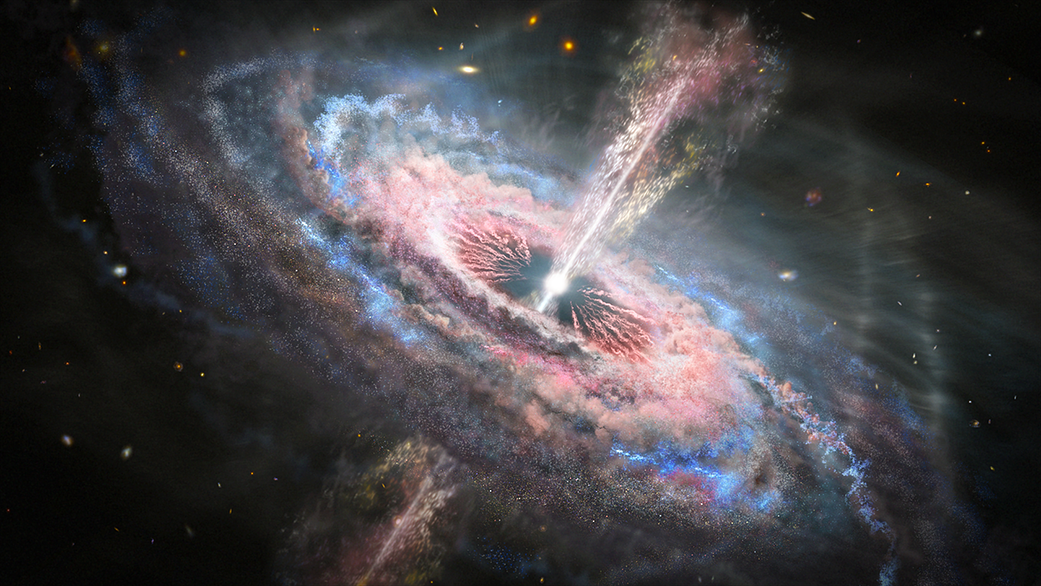
\includegraphics[scale=0.25]{galaxy.png}
    \caption{Galaxy Image Center}
    \label{fig::galaxy:top}
\end{figure}

\begin{figure}[ht]
    \centering
    \begin{minipage}[b]{0.4\textwidth}
        \caption{Caption Over}
        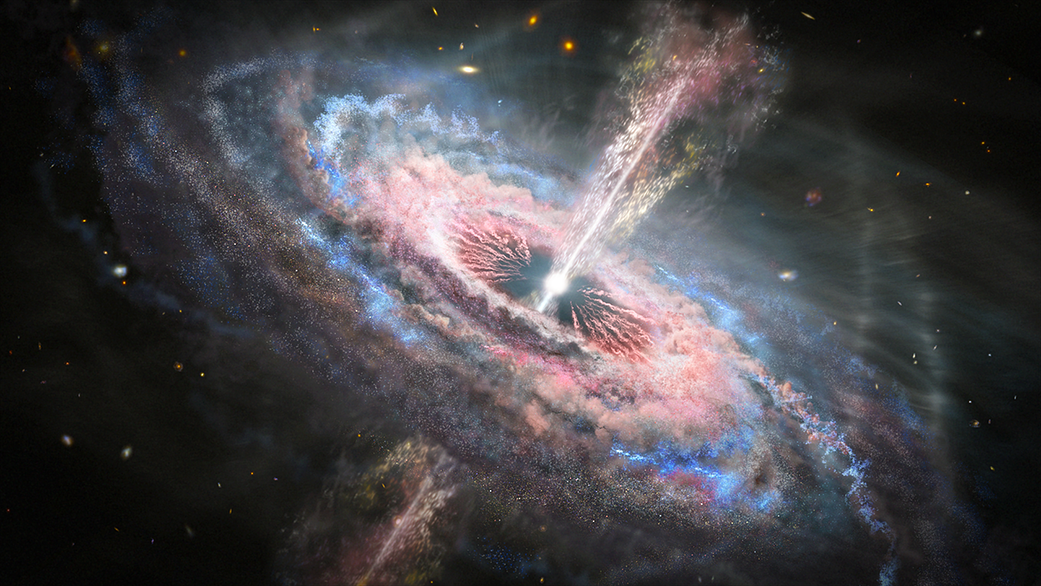
\includegraphics[width=\textwidth]{galaxy.png}
        \label{fig::galaxy:left}
    \end{minipage}
    \hfill
    \begin{minipage}[b]{0.4\textwidth}
        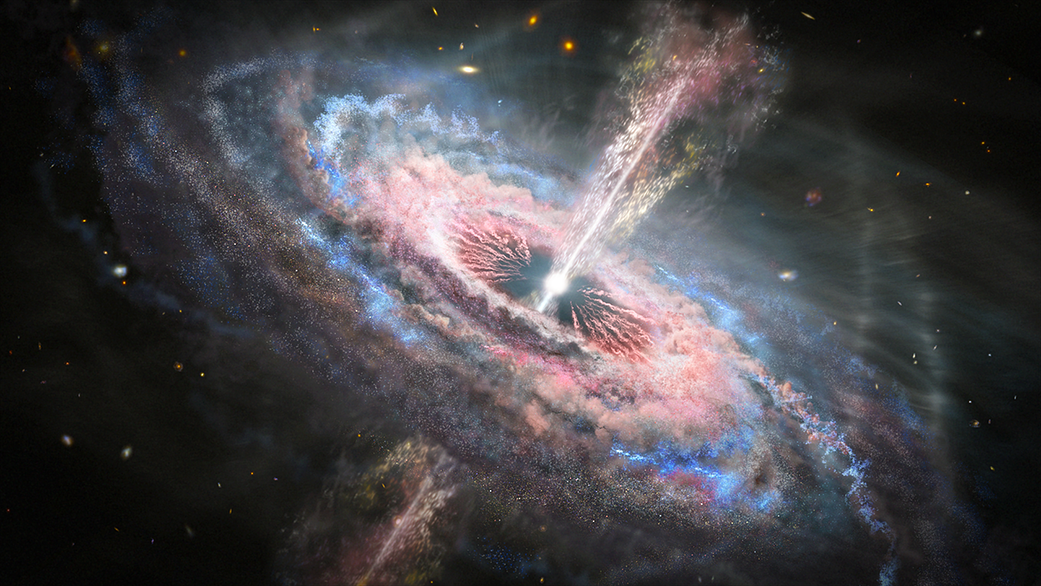
\includegraphics[width=\textwidth]{galaxy.png}
        \caption{Caption Under}
        \label{fig::galaxy:right}
    \end{minipage}
\end{figure}